\documentclass[conference]{IEEEtran}
\IEEEoverridecommandlockouts
% The preceding line is only needed to identify funding in the first footnote. If that is unneeded, please comment it out.
\usepackage{cite}
\usepackage{amsmath,amssymb,amsfonts}
\usepackage{algorithmic}
\usepackage{graphicx}
\usepackage{textcomp}
\usepackage{xcolor}
\def\BibTeX{{\rm B\kern-.05em{\sc i\kern-.025em b}\kern-.08em
T\kern-.1667em\lower.7ex\hbox{E}\kern-.125emX}}
\begin{document}

\title{Crop Classification based on Soil Information}

\makeatletter
\newcommand{\linebreakand}{%
  \end{@IEEEauthorhalign}
  \hfill\mbox{}\par
  \mbox{}\hfill\begin{@IEEEauthorhalign}
}
\makeatother

\author{
\IEEEauthorblockN{Krish L Sharma}
\IEEEauthorblockA{\textit{School Of Computer Science and Engineering} \\
\textit{Vellore Institute Of Technology, Bhopal}\\
Bhopal, India \\
krish.sharma2020@vitbhopal.ac.in}
\and
\IEEEauthorblockN{Yashaswi Patel}
\IEEEauthorblockA{\textit{School Of Computer Science and Engineering} \\
\textit{Vellore Institute Of Technology, Bhopal}\\
Bhopal, India \\
yashaswi.patel2020@vitbhopal.ac.in}
\linebreakand
\IEEEauthorblockN{Ankur Jain}
\IEEEauthorblockA{\textit{School of Computing Science and Engineering} \\
\textit{Vellore Institute of Technology, Bhopal}\\
Bhopal, India \\
ankur.jain@vitbhopal.ac.in}
}

\maketitle

\begin{abstract}
This document is a model and instructions for \LaTeX.
This and the IEEEtran.cls file define the components of your paper [title, text, heads, etc.]. *CRITICAL: Do Not Use Symbols, Special Characters, Footnotes, 
or Math in Paper Title or Abstract.
\end{abstract}

\begin{IEEEkeywords}
component, formatting, style, styling, insert
\end{IEEEkeywords}

\section{Introduction}
This document is a model and instructions for \LaTeX.
Please observe the conference page limits. 

\section{Literature Review}
In \cite{b1} paper, it was observed that C. Chen and H. Mcnairn optimised the neural network design process by using the hierarchical procedure. The hierarchical procedure helps in finding the best network structure and the optimal network parameters. These questions of the neural network are very important and difficult to find as it is a trial and error-based finding which is impractical to try all the combinations. Hence, the hierarchical procedure is being used. The procedure is as follows:

\begin{enumerate}
    \item Keep the learning rate and the momentum as constant and try all the design structures and training iterations.
    \item After finding the best design structure, move forward on trying all the learning rate and momentum combinations.
\end{enumerate}

The study has been done on 7 different models with 3 one-layered models and 4 two-layered models. Out of the 7 models, 2 models were found optimal which were: \emph{\textbf{6-18-3}} and \emph{\textbf{6-12-6-3}}. Among the two models, \emph{\textbf{6-12-6-3}} was selected as the best model because it had the highest accuracy and was more stable amongst the models for classification. Moreover, the training had a dynamic range of training time which can be easily optimised. The conclusion being that 2 hidden layer architecture was more stable and giving high accuracy if they have the following rules for the hidden layers:

\begin{enumerate}
    \item The size of the first hidden layer should be greater than that of the input layer and the second hidden layer.

    \item The second hidden layer should be less than that of the first hidden layer but not close to the output layer size.
\end{enumerate}

Moreover, \cite{b2} has tried all the available neural networks with a range of numbers [1,10] of hidden layers based on classification. According to the study, it has been concluded that all the neural networks for classification that have been used are made of 2 hidden layers and with sigmoid function. The paper has trained all types of the neural networks with 70\% training data, 15\% validation data and 15\% testing data. Trying to achieve more accuracy they tried to change the number of hidden layers with a range of 10 hidden layers. The study has trained all with combinations of number of hidden layers and finally came to a conclusion that 10 layered neural network has shown promising accuracy and optimality but expensive with respect to computational due to multiple layers.

This \cite{b3} study aimed classification by using three different classifications. These models were logistic regression, artificial neural networks, and a stacking model. It was observed that a total of 34 features were obtained out of which 30 important features were selected. The authors evaluated the performance of the proposed approach using various metrics, including accuracy, precision, recall, and F1-score. The stacking model combined the outputs of the logistic regression and ANN models. The results showed that the Stacking Model outperformed the other two algorithms.

\begin{figure}[h!]
    \centering
    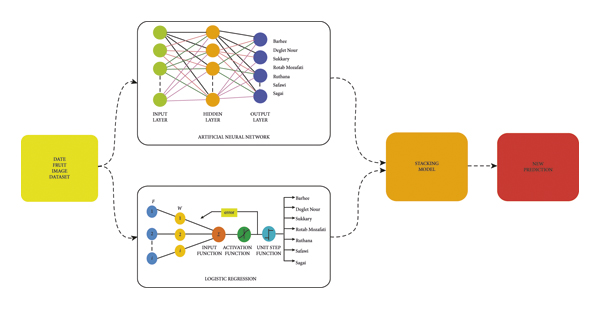
\includegraphics{StackingModelFlowChart.jpg}
    \caption[width=8cm]{\cite{b3} Stacking Model Flowchart}
    \label{fig:StackingModelFlowchart}
\end{figure}

For classifying different plants and crops, which include barley, pomegranate, cherries, grapes, pistachio, red pepper, tomato, wheat, cotton, apricot, sunflower, tangerine, corn, beans and apple, this \cite{b4} study relied heavily on a pre-trained Convolutional Neural Network model. For the classification task, the authors employed convolution neural network, and support vector machine techniques. Instead of connecting each node in the current layer to the nodes in the previous layer, each node in this case was only connected to a local region of the input volume. The CNN model was observed to learn and optimise the filters in each layer via the back-propagation mechanism. The classification performance of a CNN-based approach was compared to that of an SVM classifier with different kernels and features. SVM classifier was tested with RBF and polynomial kernels, as well as various types of features, such as four-connected LBP, GIST with 12 orientations per scale, and 4 blocks methods. The accuracy rates fluctuated between 69.81\% to 97.47\%. It was discovered that features learned from the CNN framework outperform state-of-the-art solutions that make use of carefully selected hand-crafted features. Even with different kernels and features, the SVM classifier falls short of the performance of our CNN-based approach.

The purpose of this \cite{b5} study was to classify wheat crops using multi-temporal images. The study looked at two approaches for the effective classification of multi-temporal images: Multi Label Classification(MLC) with different strategies:
\begin{enumerate}
    \item Sequential MLC
    \item PCA-based MLC
    \item Iterative-based MLC
    \item ANN
\end{enumerate}
In terms of feasibility of implementation, completeness of classification, and labelling reliability, Iterative-based MLC was found to be superior to the other two MLC strategies. ANN demonstrated the ability to perform classification in just a single stretch, whereas traditional MLC produced significantly less reliable results. Despite the fact that Iterative-based MLC resulted in a significant improvement in classification over MLC.

\section{Objective}
The following are the objective of our study on classification of the crops based on the soil nutrients:

\begin{enumerate}
    \item \emph{\textbf{Building an accurate model}}: The first objective s to build a deep learning-based neural network model that accurately predicts the type of crop that can be grown on a given piece of land based on the soil information extracted from the land. The model should be able to learn the complex relationships between the soil characteristics and the crop types and generalize well to new unseen data.

    \item \emph{\textbf{Improving crop yield}}: The second objective is to improve crop yield by providing accurate information about the types of crops that can be grown on a given piece of land. By accurately predicting the crop type, farmers can make informed decision about which crops to plant on their land, leading to better crop yields and potentially increased profitability. This can also have environmental benefits by reducing the used of fertilizers and other inputs that may be unnecessary for certain crops.
\end{enumerate}

\section{Problem Formulation}
Let X be a set of n samples, where each sample $x_{i}$ represents soil information extracted from a piece of land. Each sample $x_{i}$ contains m feature \{$x_{i_1}, x_{i_2}, ..., x_{i_m}$\}, where each feature represents a soil characteristics such as pH level, nutrient content, etc.

\begin{figure}[h!]
    \centering
    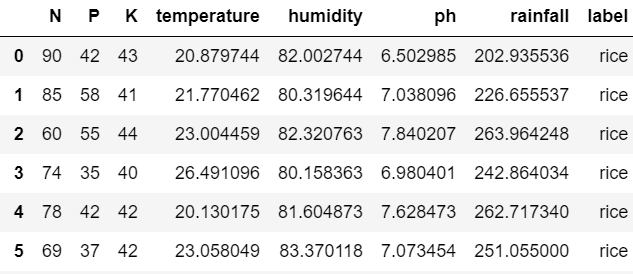
\includegraphics[width = 8cm] {Dataset.png}
    \caption{Dataset}
    \label{fig:Dataset}
\end{figure}

Let Y be a set of n labels, where each label $y_{i}$ represents the type of crop that can be grown on the corresponding land. The label $y_{i}$ belongs to a set of k possible classes \{$y_{1}, y_{2}, ... y_{k}$\}, where each class represents a specific crop as seen in Fig. 2.

\begin{figure}[h!]
    \centering
    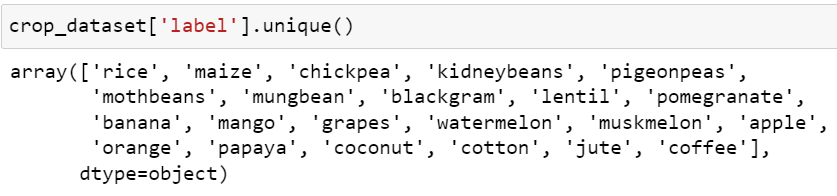
\includegraphics[width = 8cm] {labels.png}
    \caption{Crops for Classification}
    \label{fig:Crops for Classification}
\end{figure}

The objective is to build a deep learning-based neural network model that can learn the mapping between the soil information X and the crop label Y, and predict the correct crop label for new samples of soil information.

Let $f(X, \theta)$ be a neural network model with parameters $\theta$. The model takes as input a sample $x_{i}$ from X and outputs a probability distribution over the k possible classes. The predicted label for $x_i$ is the class with the highest probability in the output distribution.

The model is trained by minimizing a loss function $L(Y, f(X, \theta)$, which measures the difference between the predicted probability distribution and the true label $y_i$. A common choice for the loss function is the categorical cross-entropy loss:

\[L(Y, f(X, \theta)) = -\sum_i^k y_{i} log(f(x_{i}, \theta))\]

where $f(x_i, \theta)$ is the predicted probability distribution for $x_i$ and $y_i$ is the true label for $x_i$ encoded as a one-hot encoder.

The parameters $\theta$ are updated using gradient descent or a variant of it, such as Adam. The model is trained using a training set of labelled soil samples and evaluated on a separate validation set to monitor its performance and prevent overfitting. Once the model is trained and validated, it can be used to predict the crop label for new unseen soil samples.

\section{Methodology}
The methodology to solve the problem of classifying crops based on soil information extracted from land using a deep learning-based neural network model can be broken down into the following steps:

\begin{figure}[h!]
    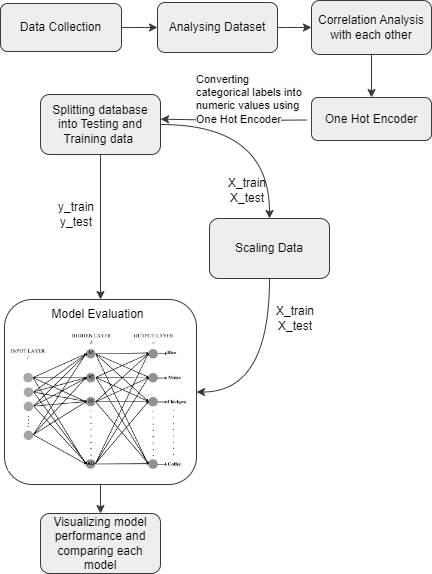
\includegraphics[width = 8cm] {flowchart.drawio (1).png}
    \caption{Flowchart of the model}
    \label{fig:Flowchart of the model}
\end{figure}

\subsection{\emph{\textbf{Data collection and preprocessing}}}
The first step is to collect soil data and corresponding crop labels for a variety of lands. This can be done by taking soil samples from different locations and testing them in a laboratory to extract various soil characteristics such as pH level, nutrient content, etc.
\begin{figure}[h!]
    \centering
    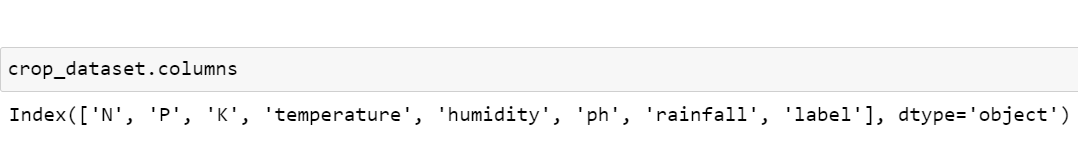
\includegraphics[width = 8cm] {columns.png}
    \caption{Different soil characteristics}
    \label{fig:Different soil characteristics}
\end{figure}

The crop labels can be obtained by surveying the lands or by consulting with local farmers. Once the data is collected, it needs to be preprocessed, which may involve cleaning, normalizing, and splitting it into training, validation, and testing sets.

\subsection{\emph{\textbf{Model selection and design}}}
The next step is to select an appropriate deep learning-based neural network model and design its architecture. The model architecture may involve selecting the number and type of layers, the number of neurons in each layer, and the activation functions to be used. The model architecture can be optimized through hyperparameters (node size of each layer, number of epochs, learning rate, etc.) tuning to improve its performance. In this case we have used 8 Models with a combination of sigmoid, tanh and relu activation function in the output layer and the hidden layer. The size of hidden layer is 22 which is same as that of the output layer. Moreover, the hyperparameters such as number of epochs and metrics are taken 200 and accuracy, respectively.

\begin{figure}[h!]
    \centering
    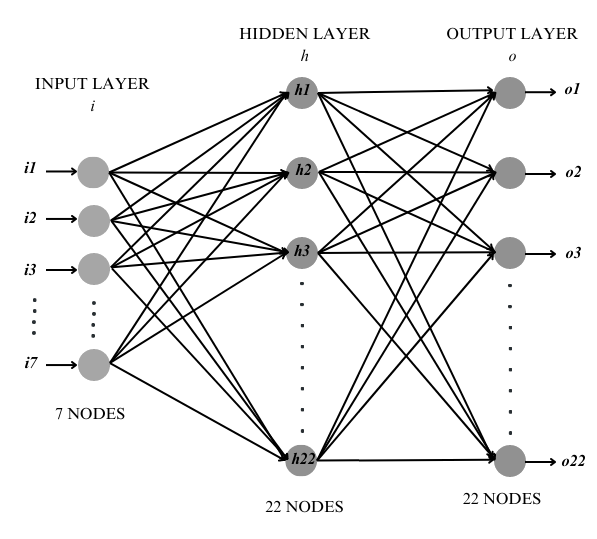
\includegraphics[width = 8cm] {7 nodes.png}
    \caption{Neural Network Architecture}
    \label{fig:Neural Network Architecture}
\end{figure}

\subsection{\emph{\textbf{Training and validation}}}
The model is then trained using the training set and validated using the validation set. During training, the model learns the complex relationships between the soil characteristics and the crop types. The model's performance is monitored during training and validation using metrics such as accuracy, precision, recall, and F1 score. The training can be stopped when the model's performance on the validation set starts to deteriorate, indicating overfitting. The training data is 80\% and the testing data is 20\% of the data. 

\begin{figure}[h!]
    \centering
    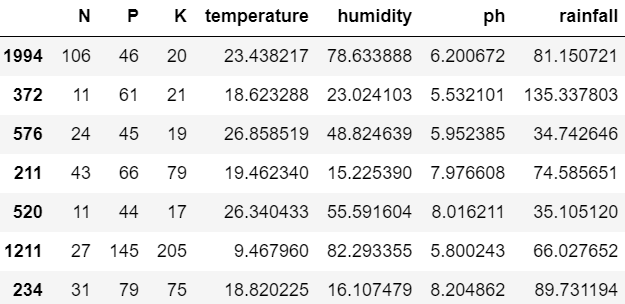
\includegraphics[width = 8cm] {x_train.png}
    \caption{Training Data}
    \label{fig:Training Data}
\end{figure}

\begin{figure}[h!]
    \centering
    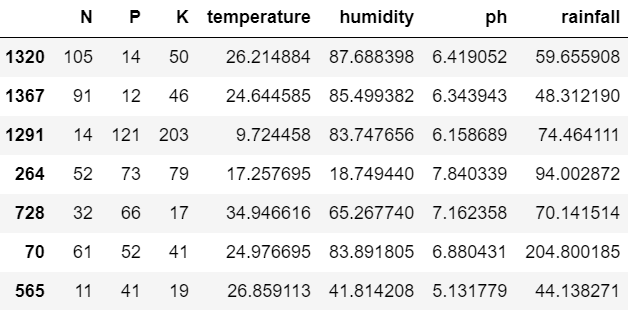
\includegraphics[width = 8cm] {x_test.png}
    \caption{Testing Data}
    \label{fig:Testing Data}
\end{figure}


\subsection{\emph{\textbf{Model evaluation}}}
Once the model is trained, it is evaluated using the testing set. This gives an estimate of the model's performance on unseen data. The evaluation metrics can be compared to those obtained during training and validation to check for any significant drops in performance.

\subsection{\emph{\textbf{Model deployment}}}
After the model is trained and evaluated, it can be deployed to predict the crop type for new soil data. The deployment can be done using a web or mobile application that takes in the soil data as input and returns the predicted crop type as output.

\subsection{\emph{\textbf{Model maintenance and updates}}}
The final step is to maintain and update the model as new data becomes available. The model's performance can be monitored regularly to check for any deterioration in its performance, and updates can be made to the model's architecture or hyperparameters as necessary. Additionally, new data can be added to the training set to improve the model's performance over time.  

Moreover, this model can be used on IoT based devices to make it more reachable to the farmers. Also, same can be used to make a recommendation system using Fuzzy Logic system. This will help the farmers to gain good knowledge about their farmlands. We can fuse the weather and climate pattern details to the dataset to upgrade the model into recommendation system.


\section{Result}
We have applied in total 8 models and in \emph{figure} we can see the graph showing the performance of each model. For each model the graph on left shows the accuracy curve and on the right the loss curve.

\begin{figure}[htp]
    \centering
    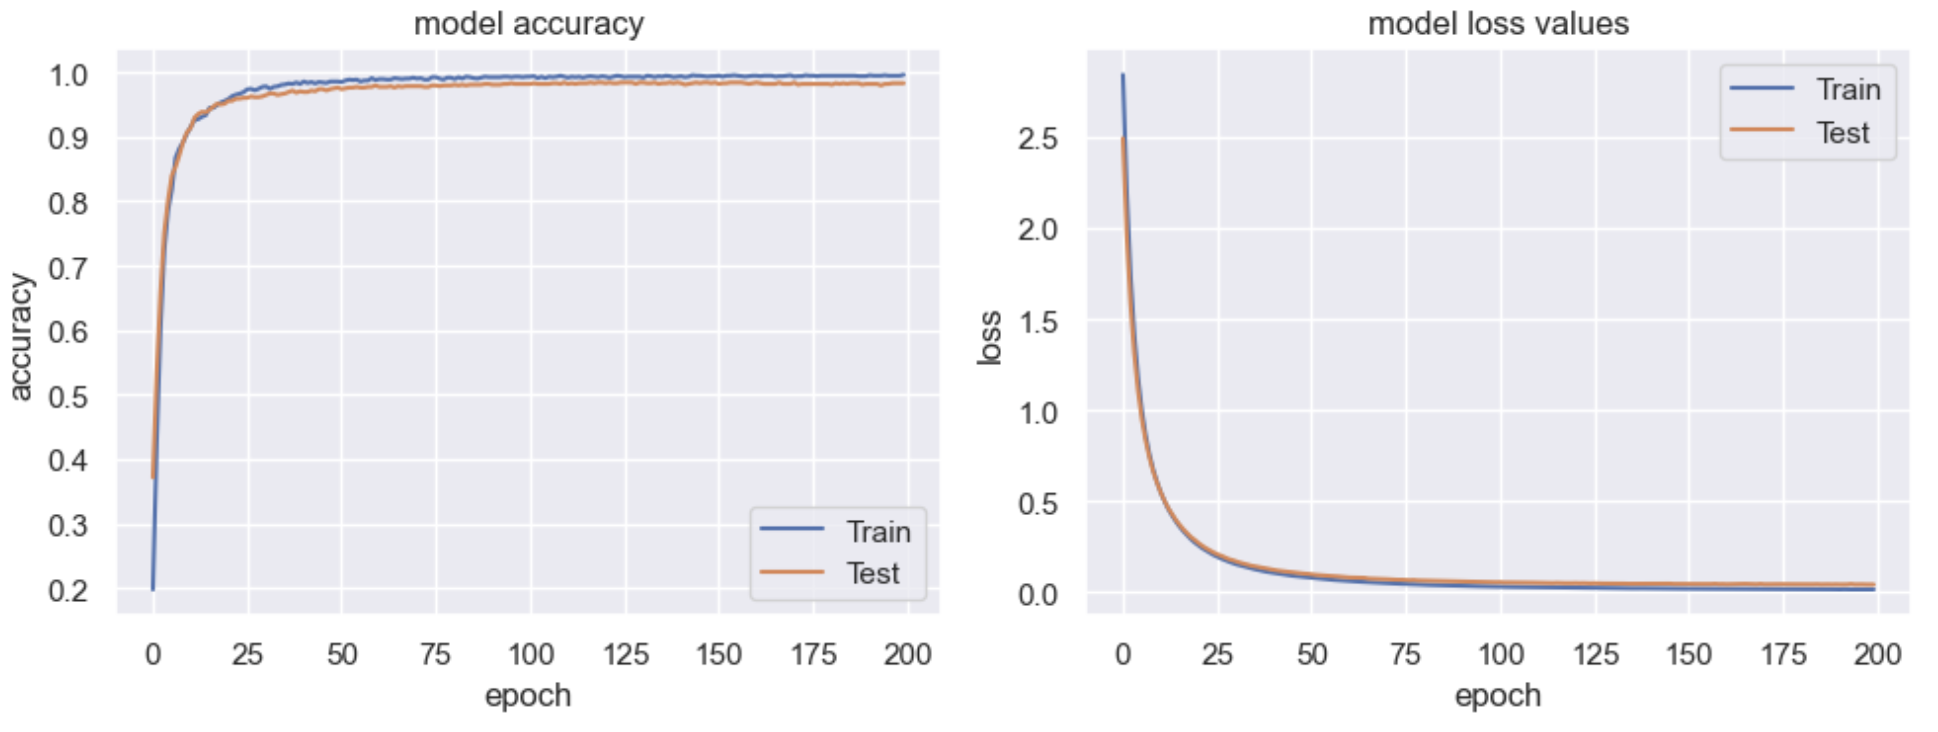
\includegraphics[width = 8cm] {Model1Performance.png}
    \caption{Model 1 Performance}
    \label{fig:Model1Performance}
\end{figure}

\begin{figure}[htp]
    \centering
    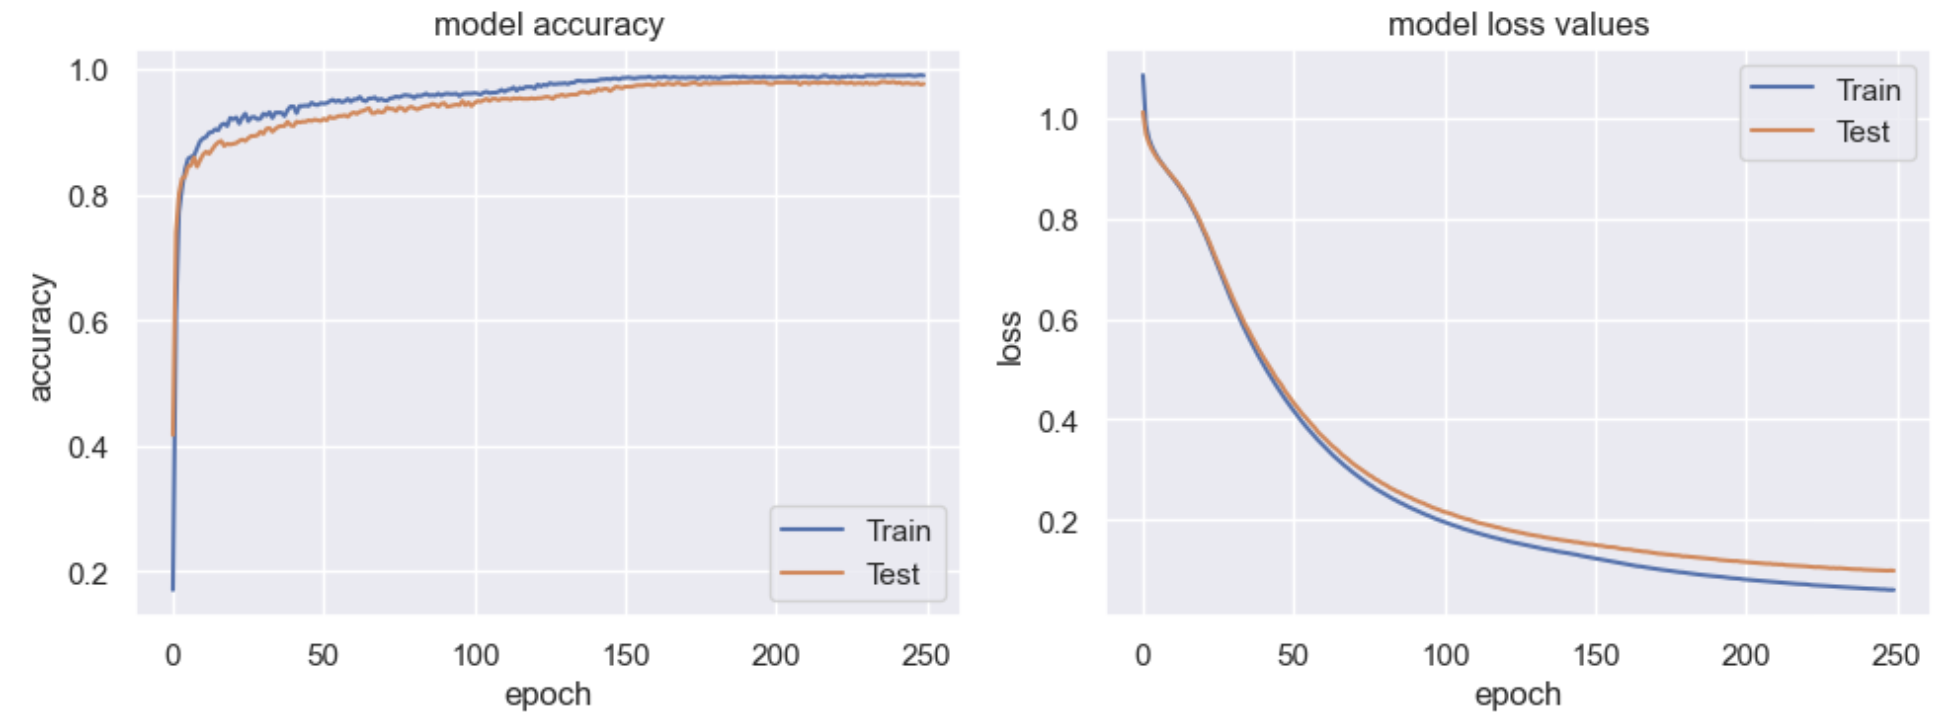
\includegraphics[width = 8cm]{Model2Performance.png}
    \caption{Model 2 Performance}
    \label{fig:Model2Performance}
\end{figure}

\begin{figure}[htp]
    \centering
    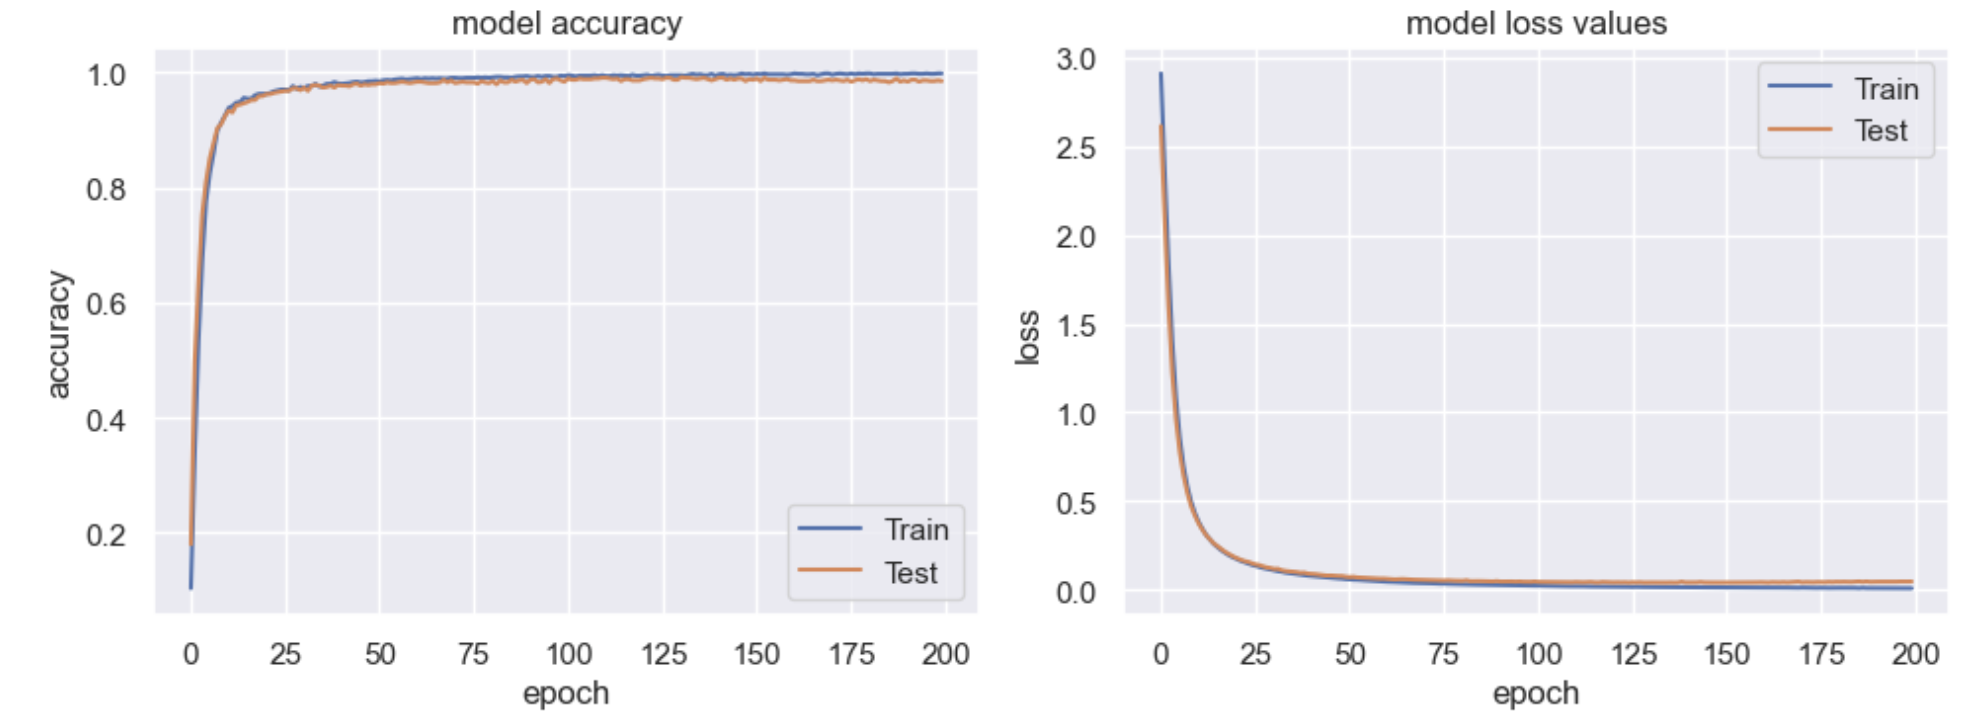
\includegraphics[width = 8cm]{Model3Performance.png}
    \caption{Model 3 Performance}
    \label{fig:Model3Performance}
\end{figure}

\begin{figure}[htp]
    \centering
    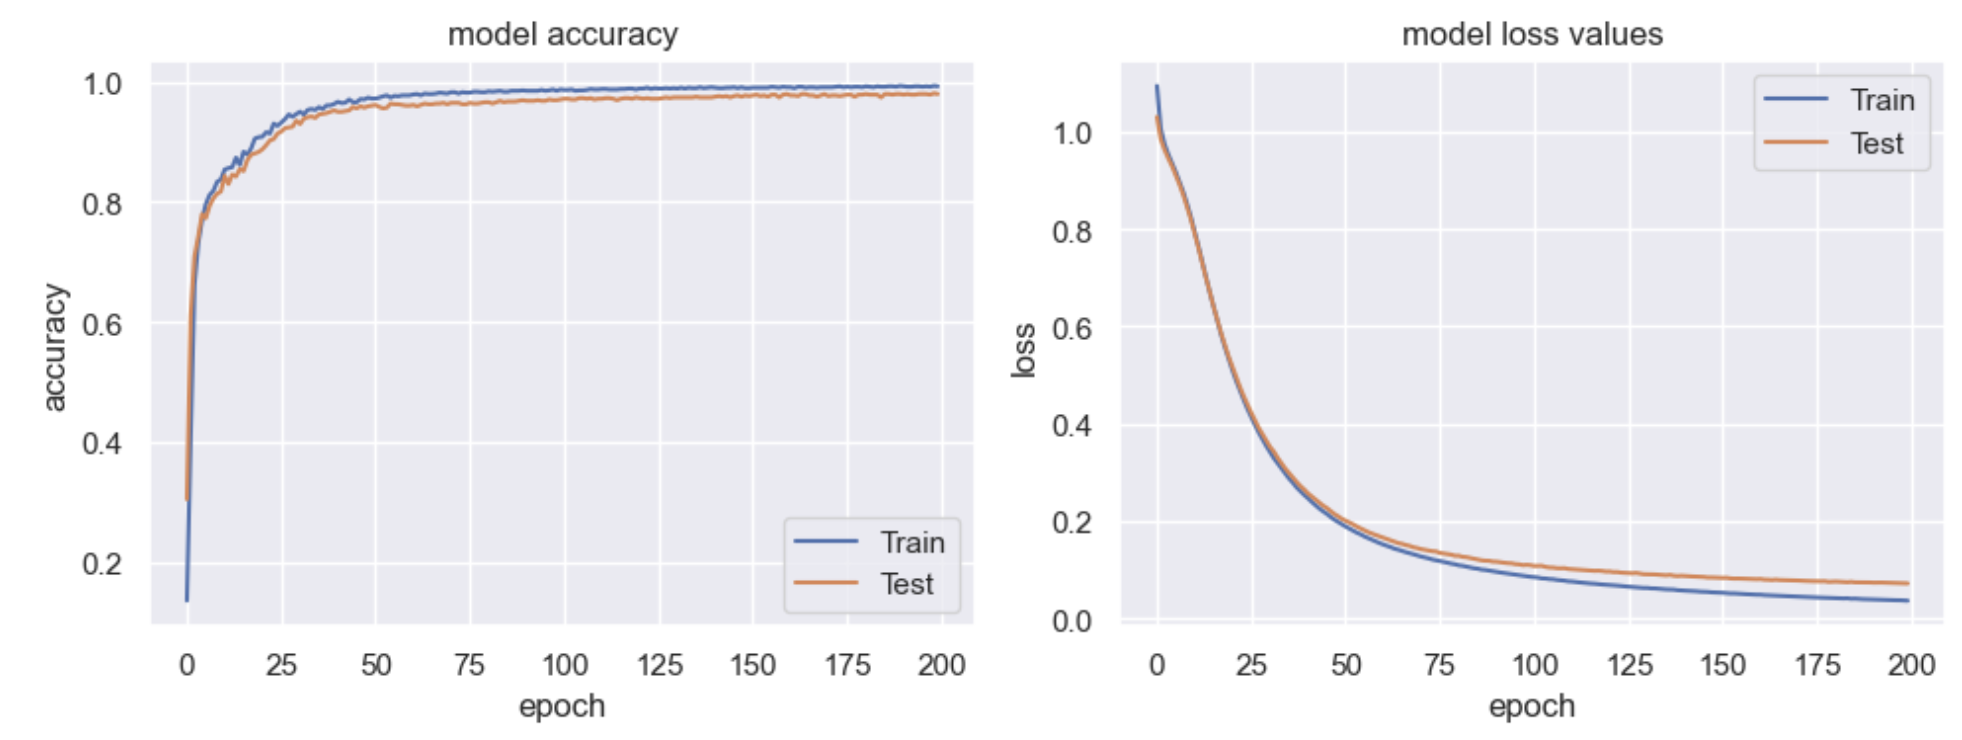
\includegraphics[width = 8cm]{Model4Performance.png}
    \caption{Model 4 Performance}
    \label{fig:Model4Performance}
\end{figure}

\begin{figure}[htp]
    \centering
    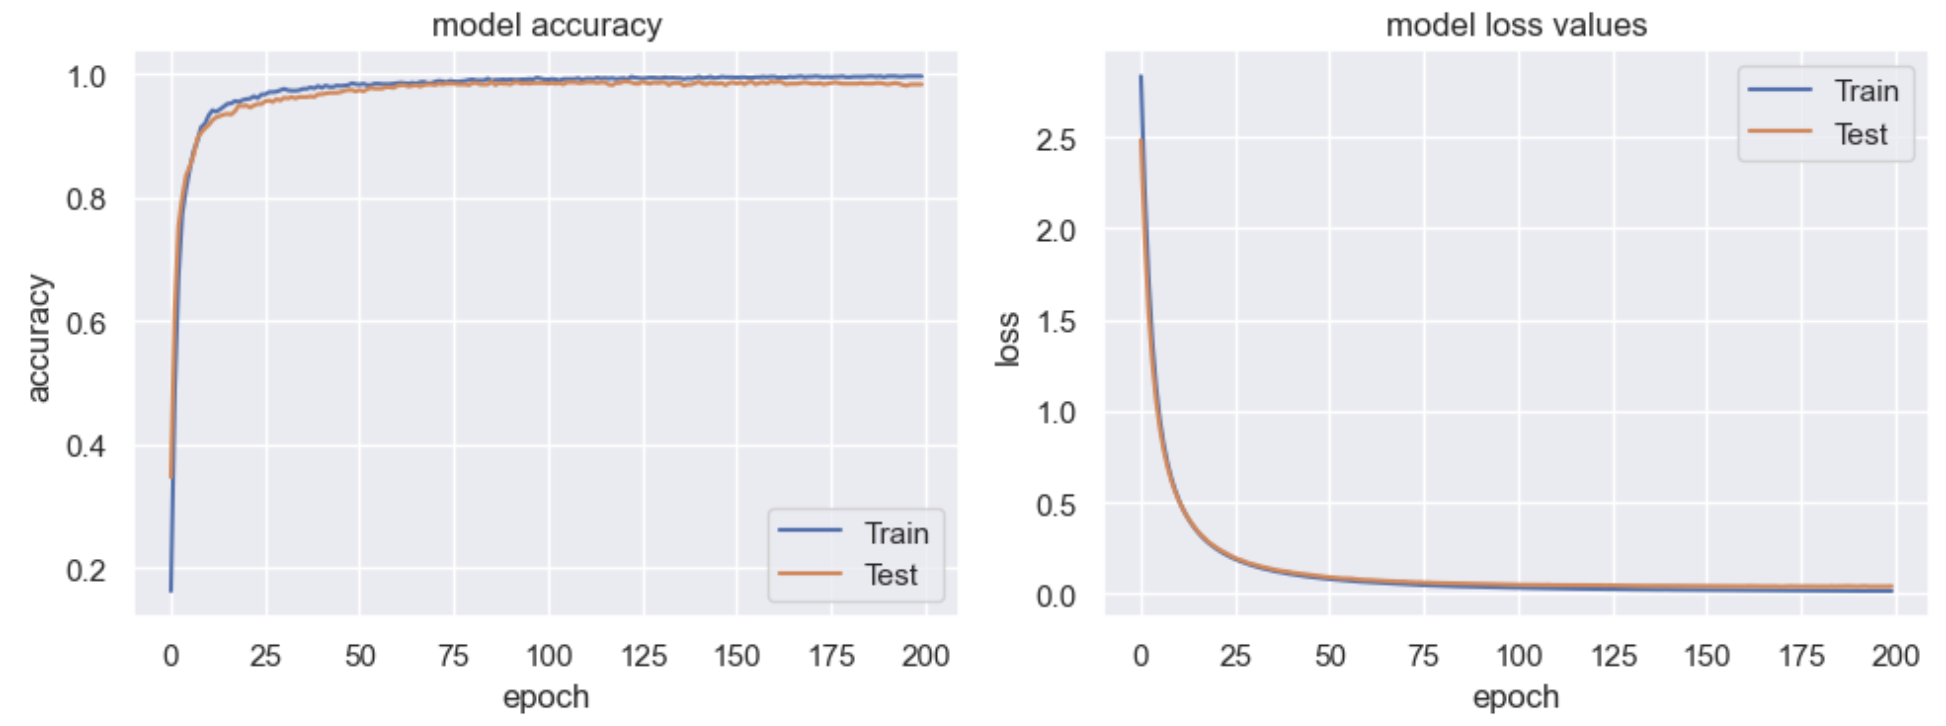
\includegraphics[width = 8cm]{Model5Performance.png}
    \caption{Model 5 Performance}
    \label{fig:Model5Performance}
\end{figure}

\begin{figure}[htp]
    \centering
    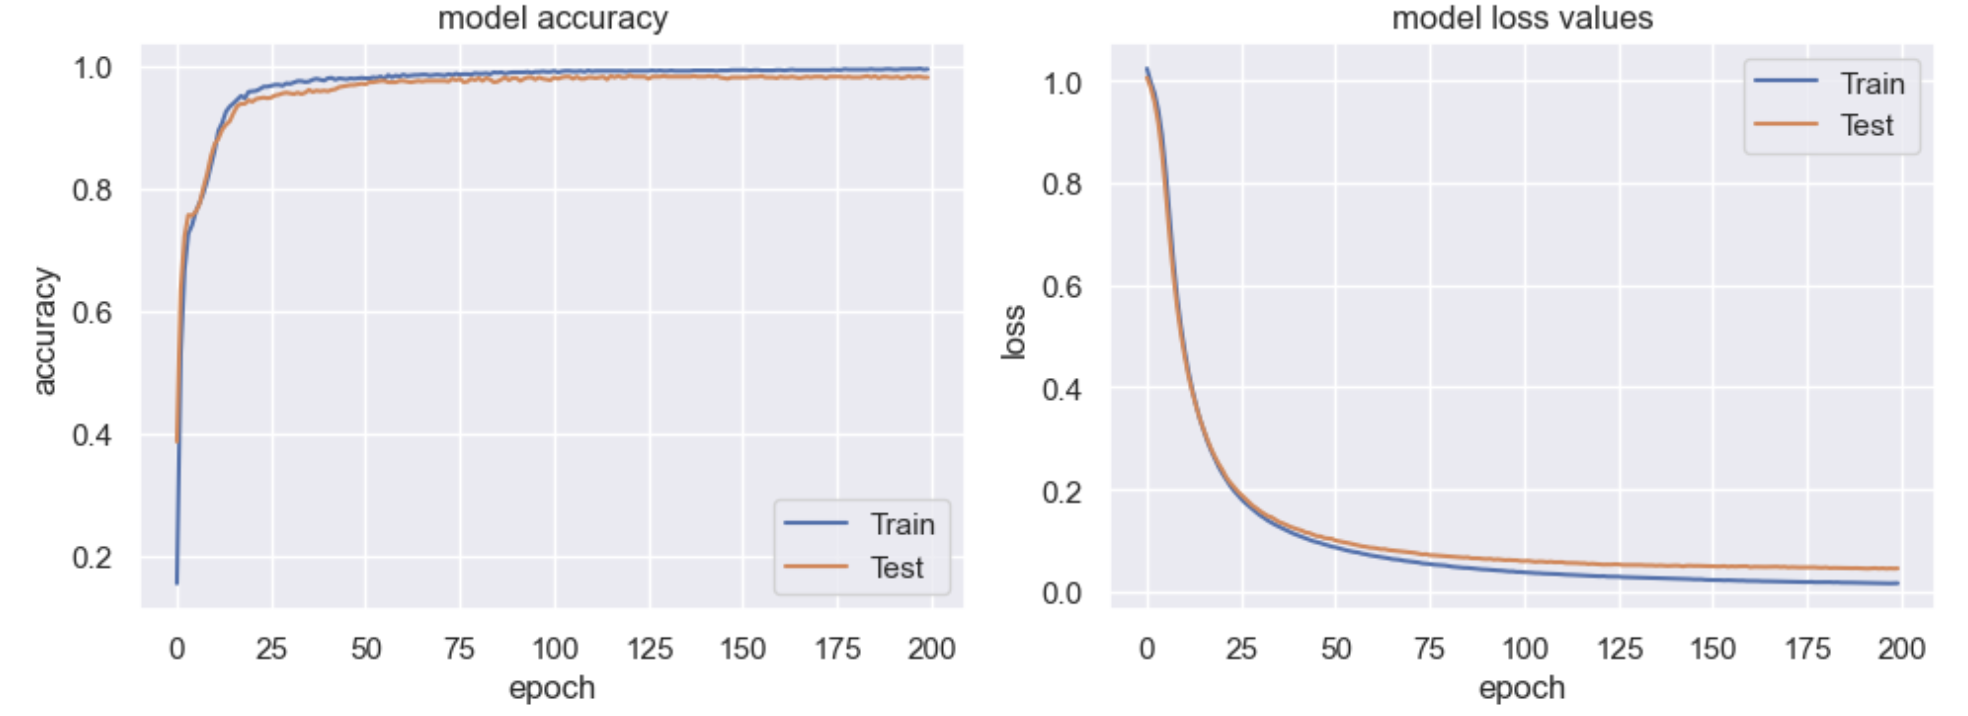
\includegraphics[width = 8cm]{Model6Performance.png}
    \caption{Model 6 Performance}
    \label{Model6Performance}
\end{figure}

\begin{figure}[htp]
    \centering
    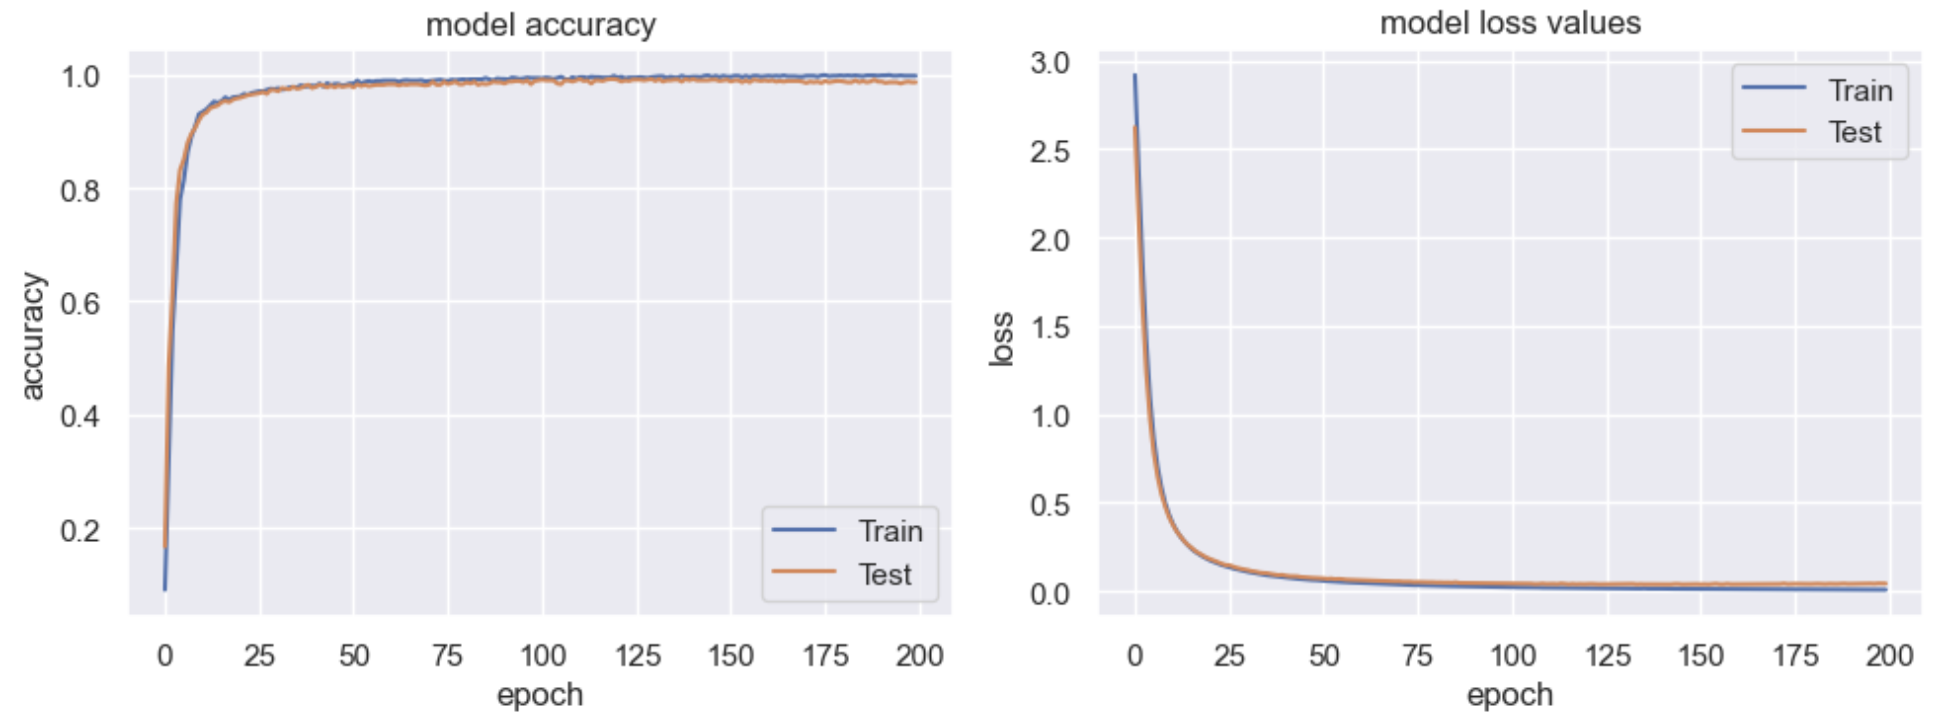
\includegraphics[width = 8cm]{Model7Performance.png}
    \caption{Model 7 Performance}
    \label{fig:Model7Performance}
\end{figure}

\begin{figure}[htp]
    \centering
    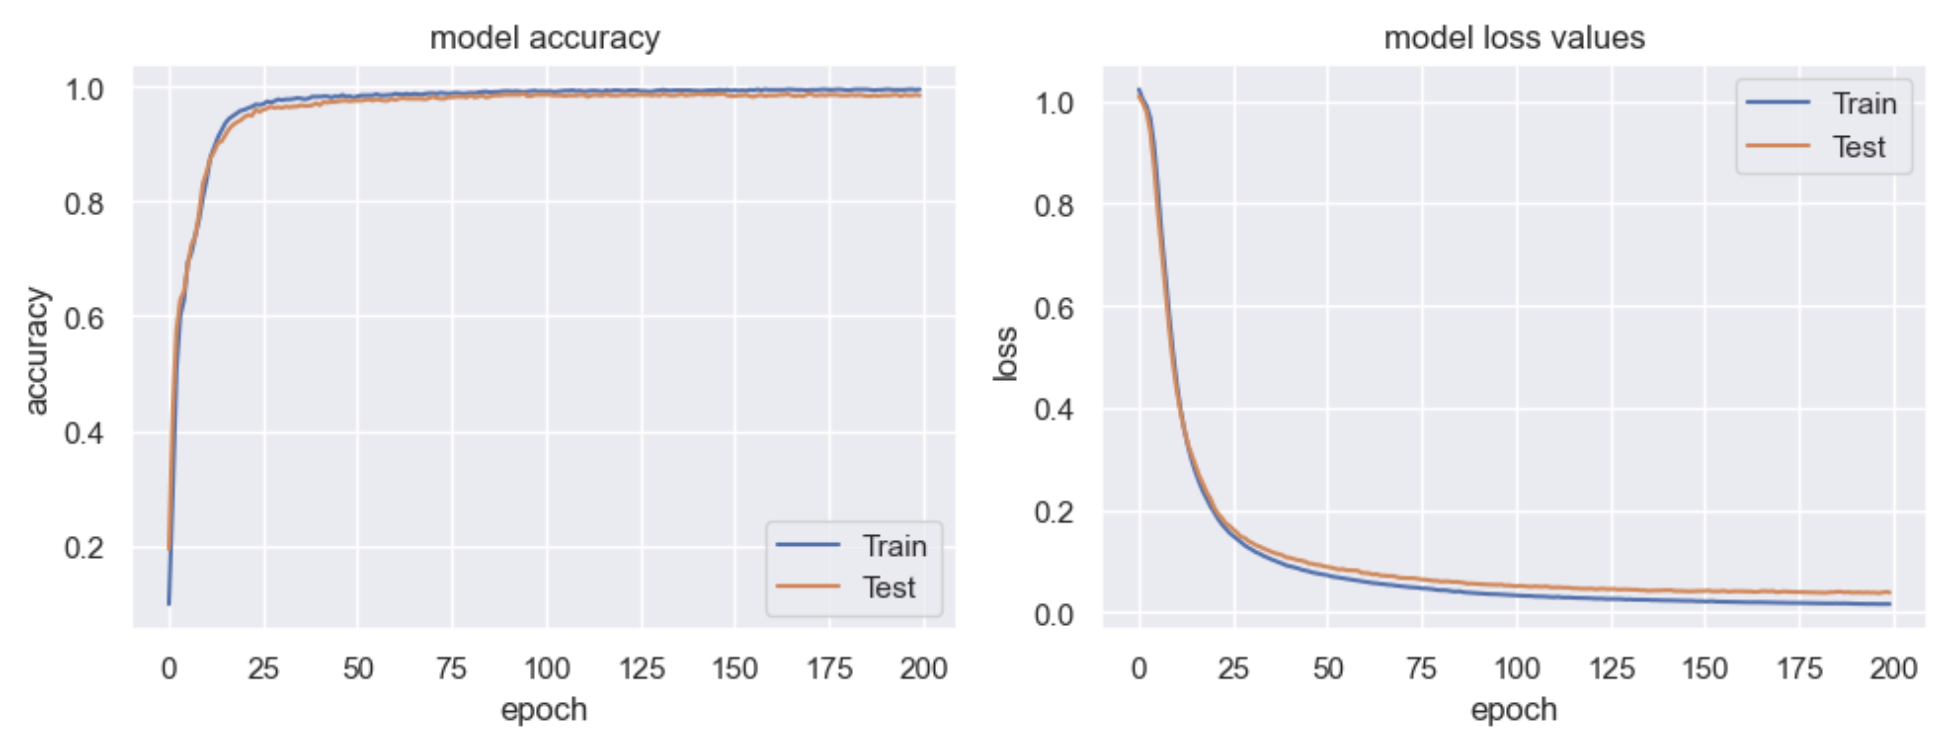
\includegraphics[width = 8cm]{Model8Performance.png}
    \caption{Model 8 Performance}
    \label{fig:Model8Performance}
\end{figure}

All the model performance are listed below with their accuracy:

\begin{enumerate}
    \item Tanh-Sigmoid-CategoricalCrossEntropy: Training Accuracy \textbf{99.772\%} and Testing Accuracy \textbf{98.181\%}.

    \item Tanh-Sigmoid-CategoricalHinge: Training Accuracy \textbf{98.712\%} and Testing Accuracy \textbf{97.272\%}

    \item ReLU-Sigmoid-CategoricalCrossEntropy: Training Accuracy \textbf{99.848\%} and Testing Accuracy \textbf{98.522\%}

    \item ReLU-Sigmoid-CategoricalHinge: Training Accuracy \textbf{99.091\%} and Testing Accuracy \textbf{97.5\%}

    \item Tanh-Softmax-CategoricalCrossEntropy: Training Accuracy \textbf{99.621\%} and Testing Accuracy\textbf{98.522\%}

    \item Tanh-Softmax-CategoricalHinge: Training Accuracy \textbf{99.621\%} and Testing Accuracy \textbf{98.182\%}

    \item ReLU-Softmax-CategoricalCrossEntropy: Training Accuracy \textbf{99.848\%} and Testing Accuracy \textbf{98.977\%}

    \item ReLU-Softmax-CategoricalHinge: Training Accuracy \textbf{99.545\%} and Testing Accuracy \textbf{98.522\%}

\end{enumerate}

Out of all the models tried and tested we can see that models \{5, 7, 8\} are giving very promising result out of which Model 7 is the best model out of all having a very good generalization and accuracy for the given classification problem.

\section{Conclusion}

\section*{Acknowledgment}

\begin{thebibliography}{00}
\bibitem{b1} C. Chen, H. Mcnairn, ``A neural network integrated approach for rice crop monitoring''
\bibitem{b2} Abdulhamid Haidar, Haiwei Dong and Nikolaos Mavridis, ``Image-Based Date Fruit Classification''
\bibitem{b3} Murat Koklu, Ramazan Kursun, Yavuz Selim Taspinar and Ilkay Cinar, ``Classification of Date Fruits into Genetic Varieties Using Image Analysis``
\bibitem{b4} Hulya Yalcin, Salar Razavi, ``Plant Classification using Convolution Neural Network``
\bibitem{b5} C. S. Murthy, P. V. Raju and K. V. S Badrinath, ``Classification of wheat crop with multi-temporal images: performance of maximum likelihood and artificial neural networks``
\bibitem{b6} Nguyen-Thanh Son, Chi-Farn Chen, Cheng-Ru Chen, Piero Toscano, Youg-Sing Cheng, Hong-Yuh Guo, Chien-Hui Syu. ``A phenological object-based approach for rice crop classification using time-series Sentinel-1 Synthetic Aperture Radar (SAR) data in Taiwan``
\bibitem{b7} Alex O. Onojeghuo, George A. Blackburn, Qunming Wang, Peter M. Atkinson, Daniel Kindred, Yuxin Miao. ``Mapping paddy rice fields by applying machine learning algorithms to multi-temporal Sentinel-1A and Landsat data``
\bibitem{b8} Zhiyuan Pei, Songling Zhang, Lin Guo, Heather McNairn, Jiali Shang, Xianfeng Jiao. ``Rice identification and change detection using TerraSAR-X data``
\bibitem{b9} A. Beyaz, R. Ozturk, and U. Turker, ``Assessment of mechanical damage on apples with image analysis``
\bibitem{b10} Oussama Aiadi, Belal Khaldi, Mohammed Lamine Kherfi, Mohamed Lamine Mekhalfi, Abdullah Alharbi, ``Date Fruit Sorting Based on Deep Learning and Discriminant Correlation Analysis``
\bibitem{b11} Jui-Feng Yeh, Kuei-Mei Lin, Chen-Yu Lin, Jen-Chun Kang, ``Intelligent Mango Fruit Glade Classification Using AlexNet with GrabCut Algorithm``
\bibitem{b12} Puteri Khatya Fahira, Zulia Putri Rahmadhani, Petrus Mursanto, Ari Wibisono, Hanif Arief Wisesa, ``Classical Machine Learning Classification for Javanese Traditional Food Image``
\bibitem{b13} C. Arun, Akshatha Prabhu, Mohammed Zeeshan, N. Shobha Rani, ``A Study on Various Classifier Techniques Used in Image Processing``
\bibitem{b14} Ahmed Chiheb Ammari, Lazhar Khriji, Medhat Awadalla, ``HW/SW Co-‘esign for Dates Classification on Xilinx Zynq SoC``
\bibitem{b15} Adnan Ahmed Abi Sen, Nour Mahmoud Bahbouh, Ahmad B. Alkhodre, Ashwaq Mohammed Aldhawi, Fatmah Ahmad Aldham, Manar Ibrahim Aljabri, ``A Classification Algorithm for Date Fruits``
\bibitem{b16} Ghulam Muhammad, M. Shamim Hossain, Abdulsalam Yassine, ``Tree-Based Deep Networks for Edge Devices``
\bibitem{b17} Puteri Khatya Fahira, Ari Wibisono, Hanif Arief Wisesa, Zulia Putri Rahmadhani, Petrus Mursanto, Adi Nurhadiyatna, ``Sumatra Traditional Food Image Classification Using Classical Machine Learning``
\bibitem{b18} Anindita Septiarini, Hamdani Hamdani, Heliza Rahmania Hatta, Anita Ahmad Kasim, ``Image-based processing for ripeness classification of oil palm fruit``
\bibitem{b19} Hamdi Altaheri, Mansour Alsulaiman, Ghulam Muhammad, ``Date Fruit Classification for Robotic Harvesting in a Natural Environment Using Deep Learning``
\bibitem{b20} Hu-Lin Kuang, Leanne Lai Hang Chan, Hong Yan, ``Multi-class fruit detection based on multiple color channels``
\bibitem{b21} Ghulam Muhammad, ``Automatic Date Fruit Classification by Using Local Texture Descriptors and Shape-Size Features``
\bibitem{b22} A. M. Vyas, B. Talati, and S. Naik, ``Colour feature extraction techniques of fruits: a survey``
\bibitem{b23} R. Pandey, S. Naik, and R. Marfatia, ``Image processing and machine learning for automated fruit grading system: a technical review``
\bibitem{b24} I. Cinar and M. Koklu, ``Classification of rice varieties using artificial intelligence methods``
\bibitem{b25} S. Jana and R. Parekh, ``Shape-based fruit recognition and classification``

\end{thebibliography}
\vspace{12pt}

\end{document}
